\medskip
Un joaillier fabrique une bague en forme de cylindre creux. Il désire recouvrir d’or toutes les faces
de la bague. Sachant que recouvrir $1\,\text{mm}^2$ avec de l’or coûte $0,5$ francs, combien va-t-il payer pour recouvrir toute la bague~?

Arrondis le résultat au franc supérieur près.

\begin{minipage}[t]{0.45\textwidth}{
    \vspace{0pt}
    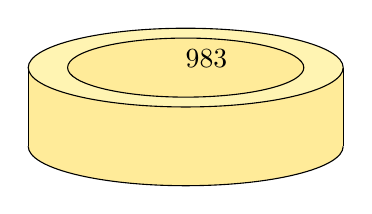
\begin{tikzpicture}
        \newcommand{\radiusx}{2}
        \newcommand{\radiusy}{.5}
        \coordinate (A) at (0,0);
        \coordinate (B) at (\radiusx,0);
        \coordinate (BB) at (-\radiusx,0);
        \coordinate (C) at (-\radiusx+0.5,0);
        \coordinate (E) at (\radiusx,-1);
        \coordinate (F) at (-\radiusx,-1);
    
    
        \fill[orange!40!yellow!40]  (B) -- (BB) -- (F) -- (E);
        \fill[orange!30!yellow!30] circle (\radiusx{} and \radiusy);
        \fill[orange!40!yellow!40] (0,-1) circle (\radiusx{} and \radiusy);
        \fill[orange!40!yellow!40] circle ({\radiusx-0.5} and {0.25*(\radiusx-0.5)});
        \draw[] (BB) -- (F);
        \draw[] (B) -- (E);
        \draw circle (\radiusx{} and \radiusy);
      \draw (-2,-1) arc[start angle=-180, end angle=0, x radius=\radiusx, y radius=\radiusy];
        \draw circle ({\radiusx-0.5} and {0.25*(\radiusx-0.5)});
        \tkzDrawSegment[dashed,dim={{$9$\,mm},20pt,}](A,B);
        \tkzDrawSegment[dashed,dim={{$8$\,mm},-20pt,}](A,C);
        \tkzDrawSegment[dashed,dim={{$3$\,mm},15pt,}](B,E);
    \end{tikzpicture}

    Croquis : bague vue latéralement
    }
    \end{minipage}
    \hfill
    \begin{minipage}[t]{0.45\textwidth}{
    \vspace{0pt}
    \begin{tikzpicture}
        \coordinate (O) at (0,0);
        \tkzDefCircle[R](O, 2) \tkzGetPoint(B);
        \tkzDrawCircle[color=black,fill=orange!40!yellow!40](O,B);
        \tkzDefCircle[R](O, 0.75) \tkzGetPoint(C);
        \tkzDrawCircle[color=black,fill=white](O,C);
        \tkzDrawSegment[dashed,dim={{$8$\,mm},60pt,}](O,C);
        \tkzDrawSegment[dashed,dim={{$9$\,mm},-60pt,}](O,B);
        \end{tikzpicture}
        
        Croquis : bague vue de dessus ou de dessous
    }
\end{minipage}


